\documentclass[landscape]{slides}

% --- Core Packages ---
\usepackage[landscape,margin=0.7in]{geometry}
\usepackage{amsmath,amssymb}
\usepackage{xcolor}
\usepackage{tcolorbox}
\usepackage{tikz}
\usetikzlibrary{positioning,calc,shapes.geometric,backgrounds}
\usepackage{booktabs}
\usepackage{colortbl}
\usepackage{array}
\usepackage{tabularx}
\usepackage{fontawesome5}
\usepackage{fancyhdr}

% --- Custom Color Palette ---
\definecolor{NavyDark}{RGB}{15,32,67}
\definecolor{TealAccent}{RGB}{0,136,145}
\definecolor{CoralAccent}{RGB}{225,112,85}
\definecolor{CardBg}{RGB}{245,247,251}
\definecolor{BorderGray}{RGB}{210,218,226}
\definecolor{TextDark}{RGB}{35,45,60}
\definecolor{TableHeadBg}{RGB}{20,40,80}
\definecolor{RowAltBg}{RGB}{240,244,248}

% --- Header and Footer Setup ---
\pagestyle{fancy}
\fancyhf{}
\fancyhead[L]{\color{NavyDark}\bfseries\small \faLayerGroup~~VERTEX DATA OS --- Technical Briefing}
\fancyhead[R]{\color{TealAccent}\bfseries\small Enterprise Architecture Review}
\fancyfoot[L]{\color{TextDark}\small Vertex Systems Engineering}
\fancyfoot[R]{\color{NavyDark}\bfseries\small Slide \thepage}
\renewcommand{\headrulewidth}{0.8pt}
\renewcommand{\footrulewidth}{0.4pt}

% --- Custom Macros ---
\newcommand{\slidetitle}[1]{%
  {\Large\bfseries\color{NavyDark} #1}\par\vspace{0.3em}%
  {\color{TealAccent}\hrule height 2pt}\vspace{0.6em}%
}

\newcommand{\sectionbanner}[2]{%
  \begin{center}
    \vspace*{1.2em}
    \begin{tcolorbox}[colback=NavyDark,colframe=TealAccent,arc=4pt,boxrule=1.5pt,center,width=0.9\textwidth]
      \centering
      \vspace{0.4em}
      {\Huge\bfseries\color{white} #1}\par\vspace{0.5em}
      {\large\color{TealAccent}\bfseries #2}
      \vspace{0.4em}
    \end{tcolorbox}
  \end{center}
}

\begin{document}

% ==========================================
% SLIDE 1: Title Slide
% ==========================================
\begin{slide}
\begin{center}
  \vspace*{0.5em}
  \begin{tcolorbox}[colback=NavyDark,colframe=TealAccent,arc=6pt,boxrule=2pt,width=0.95\textwidth]
    \centering
    \vspace{0.6em}
    {\Huge\bfseries\color{white} VERTEX DATA OS}\par\vspace{0.4em}
    {\large\color{CoralAccent}\bfseries Next-Generation Enterprise Data Mesh \& Event Processing Platform}\par\vspace{0.2em}
    \vspace{0.4em}
  \end{tcolorbox}
  
  \vspace{1.2em}
  
  \begin{tcolorbox}[colback=CardBg,colframe=BorderGray,arc=4pt,boxrule=1pt,width=0.95\textwidth]
    \centering
    \vspace{0.3em}
    {\large\color{NavyDark}\bfseries Executive Technical Briefing \& Architecture Roadmap}\par\vspace{0.5em}
    {\color{TextDark}\small Presented by: \textbf{Dr. Elena Rostova} (Chief Data Architect) \& \textbf{Marcus Vance} (VP Systems Engineering)}\par\vspace{0.2em}
    {\color{TealAccent}\small \faServer~~Vertex Systems Engineering Group ~$\cdot$~ Q3 2026}
    \vspace{0.3em}
  \end{tcolorbox}
\end{center}
\end{slide}

% ==========================================
% SLIDE 2: Executive Summary & Agenda
% ==========================================
\begin{slide}
\slidetitle{\faList~~Executive Summary \& Presentation Agenda}

\begin{minipage}[t]{0.47\textwidth}
  \begin{tcolorbox}[colback=CardBg,colframe=TealAccent,title=\textbf{\faCheckCircle~~Executive Summary}]
    \small
    \begin{itemize}
      \item \textbf{Data Mesh Core}: Decouples centralized data monoliths into domain-owned data products.
      \item \textbf{High Throughput}: Ingests and processes 10M+ events/sec with sub-10ms end-to-end latency.
      \item \textbf{Zero-Trust Security}: Integrated ABAC governance with automated SOC2 audit compliance.
    \end{itemize}
  \end{tcolorbox}
\end{minipage}%
\hfill
\begin{minipage}[t]{0.49\textwidth}
  \begin{tcolorbox}[colback=CardBg,colframe=NavyDark,title=\textbf{\faProjectDiagram~~Presentation Agenda}]
    \small
    \begin{enumerate}
      \item \textbf{Module 1}: Architectural Foundations
      \item \textbf{Module 2}: Stream Processing \& Real-Time Pipeline
      \item \textbf{Module 3}: Empirical Performance Benchmarks
      \item \textbf{Module 4}: Enterprise Security \& Governance
      \item \textbf{Module 5}: Deployment Topology \& Roadmap
    \end{enumerate}
  \end{tcolorbox}
\end{minipage}
\end{slide}

% ==========================================
% SLIDE 3: Section Divider 1
% ==========================================
\begin{slide}
\sectionbanner{MODULE 1: ARCHITECTURAL FOUNDATIONS}{Decoupled Storage, Distributed Processing \& Data Mesh Principles}
\end{slide}

% ==========================================
% SLIDE 4: Core System Architecture & Pillars
% ==========================================
\begin{slide}
\slidetitle{\faCogs~~Core System Architecture \& Design Pillars}

\begin{minipage}[t]{0.31\textwidth}
  \begin{tcolorbox}[colback=CardBg,colframe=TealAccent,title=\textbf{\faNetworkWired~~Synapse Bus}]
    \small
    \textbf{Event Streaming}
    \begin{itemize}
      \item Distributed event log
      \item Sub-10ms streaming
      \item Multi-region replication
      \item Zero-copy memory buffer
    \end{itemize}
  \end{tcolorbox}
\end{minipage}%
\hfill
\begin{minipage}[t]{0.31\textwidth}
  \begin{tcolorbox}[colback=CardBg,colframe=NavyDark,title=\textbf{\faLock~~Policy Engine}]
    \small
    \textbf{Federated Governance}
    \begin{itemize}
      \item Fine-grained ABAC policies
      \item Dynamic PII masking
      \item Immutable audit telemetry
      \item Real-time threat filter
    \end{itemize}
  \end{tcolorbox}
\end{minipage}%
\hfill
\begin{minipage}[t]{0.31\textwidth}
  \begin{tcolorbox}[colback=CardBg,colframe=CoralAccent,title=\textbf{\faDatabase~~Meridian SQL}]
    \small
    \textbf{Polyglot Query Kernel}
    \begin{itemize}
      \item ANSI SQL compliance
      \item Vectorized engine
      \item Cross-domain acceleration
      \item Automated index tuning
    \end{itemize}
  \end{tcolorbox}
\end{minipage}
\end{slide}

% ==========================================
% SLIDE 5: Data Mesh & Domain Ownership
% ==========================================
\begin{slide}
\slidetitle{\faLayerGroup~~Data Mesh \& Domain-Driven Ownership}

\begin{minipage}[t]{0.48\textwidth}
  \begin{tcolorbox}[colback=CardBg,colframe=NavyDark,title=\textbf{\faKey~~Core Architectural Principles}]
    \small
    \begin{itemize}
      \item \textbf{Domain Ownership}: Business units own data lifecycle and schema evolution.
      \item \textbf{Data as a Product}: Clean REST/gRPC interfaces with strict SLAs.
      \item \textbf{Self-Serve Platform}: Automated provisioning of streaming topics and storage buckets.
    \end{itemize}
  \end{tcolorbox}
\end{minipage}%
\hfill
\begin{minipage}[t]{0.48\textwidth}
  \begin{tcolorbox}[colback=CardBg,colframe=TealAccent,title=\textbf{\faChartLine~~Quantifiable Business Impact}]
    \small
    \begin{itemize}
      \item \textbf{40\% Reduction} in ETL pipeline maintenance costs.
      \item \textbf{3x Faster Time-to-Market} for new analytical data products.
      \item \textbf{Zero Bottlenecks}: Eliminates centralized data engineering request backlogs.
    \end{itemize}
  \end{tcolorbox}
\end{minipage}
\end{slide}

% ==========================================
% SLIDE 6: Section Divider 2
% ==========================================
\begin{slide}
\sectionbanner{MODULE 2: STREAM PROCESSING \& PIPELINE}{High-Throughput Ingestion, Real-Time Flow \& Microservices}
\end{slide}

% ==========================================
% SLIDE 7: TikZ Diagram Slide - Real-Time Pipeline
% ==========================================
\begin{slide}
\slidetitle{\faProjectDiagram~~Real-Time Event Processing Pipeline}

\begin{center}
\resizebox{\linewidth}{!}{%
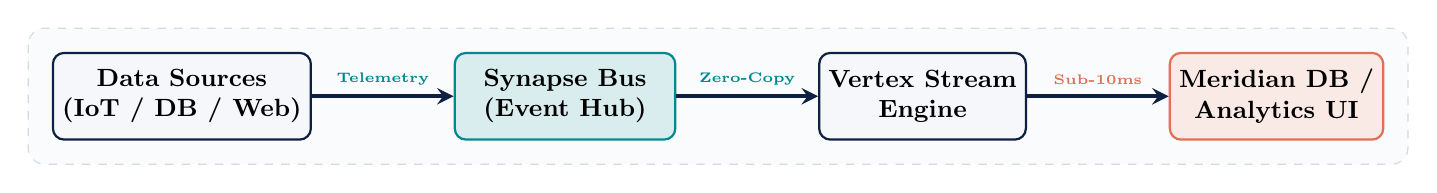
\begin{tikzpicture}[
  node distance=1.4cm and 1.8cm,
  block/.style={rectangle, draw=NavyDark, fill=CardBg, thick, rounded corners=4pt, minimum width=2.6cm, minimum height=1.1cm, align=center, font=\small\bfseries},
  accent/.style={rectangle, draw=TealAccent, fill=TealAccent!15, thick, rounded corners=4pt, minimum width=2.8cm, minimum height=1.1cm, align=center, font=\small\bfseries},
  coral/.style={rectangle, draw=CoralAccent, fill=CoralAccent!15, thick, rounded corners=4pt, minimum width=2.6cm, minimum height=1.1cm, align=center, font=\small\bfseries},
  arrow/.style={->, >=stealth, ultra thick, draw=NavyDark}
]

  % Nodes
  \node[block] (sources) {Data Sources\\(IoT / DB / Web)};
  \node[accent, right=of sources] (bus) {Synapse Bus\\(Event Hub)};
  \node[block, right=of bus] (engine) {Vertex Stream\\Engine};
  \node[coral, right=of engine] (storage) {Meridian DB /\\Analytics UI};

  % Lines / Arrows
  \draw[arrow] (sources) -- node[above, font=\tiny\bfseries\color{TealAccent}]{Telemetry} (bus);
  \draw[arrow] (bus) -- node[above, font=\tiny\bfseries\color{TealAccent}]{Zero-Copy} (engine);
  \draw[arrow] (engine) -- node[above, font=\tiny\bfseries\color{CoralAccent}]{Sub-10ms} (storage);

  % Background Box using calc
  \begin{scope}[on background layer]
    \draw[draw=BorderGray, fill=CardBg!50, dashed, rounded corners=6pt] 
      ($(sources.north west)+(-0.3,0.3)$) rectangle ($(storage.south east)+(0.3,-0.3)$);
  \end{scope}
\end{tikzpicture}
}%
\end{center}

\vspace{-0.2em}
\begin{tcolorbox}[colback=CardBg,colframe=BorderGray,arc=3pt,boxrule=1pt]
  \small\color{TextDark}\centering
  \textbf{Pipeline Flow}: Ingestion via IoT/Web gateways $\rightarrow$ Partitioned Synapse Event Hub $\rightarrow$ Parallel Stream Transformation $\rightarrow$ Real-Time Analytical Store.
\end{tcolorbox}
\end{slide}

% ==========================================
% SLIDE 8: Stream Engine Optimization
% ==========================================
\begin{slide}
\slidetitle{\faTerminal~~Stream Engine Latency \& Flow Control}

\begin{minipage}[t]{0.48\textwidth}
  \begin{tcolorbox}[colback=CardBg,colframe=TealAccent,title=\textbf{\faMemory~~Zero-Copy Memory Architecture}]
    \small
    \begin{itemize}
      \item Bypasses JVM garbage collection overhead using off-heap memory buffers.
      \item Direct kernel-to-network card transmission via RingBuffers.
      \item Sustained throughput of 12.5 million records per second per cluster node.
    \end{itemize}
  \end{tcolorbox}
\end{minipage}%
\hfill
\begin{minipage}[t]{0.48\textwidth}
  \begin{tcolorbox}[colback=CardBg,colframe=NavyDark,title=\textbf{\faCogs~~Adaptive Backpressure Control}]
    \small
    \begin{itemize}
      \item Dynamically monitors consumer queue saturation across nodes.
      \item Automatic rate-limiting feedback to ingestion edge proxies.
      \item Prevents cascading node failures during 5x traffic surges.
    \end{itemize}
  \end{tcolorbox}
\end{minipage}
\end{slide}

% ==========================================
% SLIDE 9: Section Divider 3
% ==========================================
\begin{slide}
\sectionbanner{MODULE 3: PERFORMANCE BENCHMARKS}{Empirical Evaluation, Throughput Statistics \& Latency Profiles}
\end{slide}

% ==========================================
% SLIDE 10: Table Slide - Performance Benchmarks
% ==========================================
\begin{slide}
\slidetitle{\faChartBar~~Empirical Performance Benchmark Analysis}

\small
\centering
\resizebox{\linewidth}{!}{%
\begin{tabular}{l c c c r}
\toprule
\rowcolor{TableHeadBg}
\color{white}\textbf{Benchmark Metric} & \color{white}\textbf{Legacy System} & \color{white}\textbf{Competitor X} & \color{white}\textbf{Vertex Data OS} & \color{white}\textbf{Delta} \\
\midrule
Peak Ingestion Rate & 1.2M msg/sec & 4.5M msg/sec & \textbf{12.8M msg/sec} & \color{TealAccent}\textbf{+184\%} \\
\rowcolor{RowAltBg}
End-to-End Latency (P99) & 420 ms & 85 ms & \textbf{8.4 ms} & \color{TealAccent}\textbf{10x Faster} \\
Analytical Query P95 & 14.2 sec & 3.8 sec & \textbf{0.45 sec} & \color{TealAccent}\textbf{8.4x Faster} \\
\rowcolor{RowAltBg}
Infrastructure Cost / TB & \$185.00 & \$110.00 & \textbf{\$42.00} & \color{TealAccent}\textbf{-61.8\%} \\
Failover Recovery Time & 120 sec & 25 sec & \textbf{1.8 sec} & \color{TealAccent}\textbf{92\% Faster} \\
\bottomrule
\end{tabular}
}%

\vspace{0.6em}
\begin{tcolorbox}[colback=CardBg,colframe=BorderGray,arc=3pt,boxrule=1pt]
  \small\color{TextDark}\centering
  \textbf{Benchmark Environment}: 64-Node AWS Cluster (c6i.8xlarge), 10Gbps Network, Synthetic 1KB Event Stream Payload.
\end{tcolorbox}
\end{slide}

% ==========================================
% SLIDE 11: Section Divider 4
% ==========================================
\begin{slide}
\sectionbanner{MODULE 4: ENTERPRISE SECURITY \& GOVERNANCE}{Zero-Trust Security, Data Privacy \& Regulatory Compliance}
\end{slide}

% ==========================================
% SLIDE 12: Zero-Trust Security Architecture
% ==========================================
\begin{slide}
\slidetitle{\faLock~~Zero-Trust Security \& Governance Framework}

\begin{minipage}[t]{0.31\textwidth}
  \begin{tcolorbox}[colback=CardBg,colframe=NavyDark,title=\textbf{\faKey~~IAM \& ABAC Policy}]
    \small
    \begin{itemize}
      \item Fine-grained access
      \item Micro-segmented tokens
      \item Dynamic scope check
      \item OAuth2 integration
    \end{itemize}
  \end{tcolorbox}
\end{minipage}%
\hfill
\begin{minipage}[t]{0.31\textwidth}
  \begin{tcolorbox}[colback=CardBg,colframe=TealAccent,title=\textbf{\faLock~~End-to-End Encryption}]
    \small
    \begin{itemize}
      \item TLS 1.3 in-transit
      \item AES-256-GCM at rest
      \item HSM hardware keys
      \item PII data masking
    \end{itemize}
  \end{tcolorbox}
\end{minipage}%
\hfill
\begin{minipage}[t]{0.31\textwidth}
  \begin{tcolorbox}[colback=CardBg,colframe=CoralAccent,title=\textbf{\faFile~~Compliance \& Audit}]
    \small
    \begin{itemize}
      \item SOC2 Type II certified
      \item GDPR erasure automation
      \item Immutable log storage
      \item Vulnerability scans
    \end{itemize}
  \end{tcolorbox}
\end{minipage}
\end{slide}

% ==========================================
% SLIDE 13: Section Divider 5
% ==========================================
\begin{slide}
\sectionbanner{MODULE 5: DEPLOYMENT TOPOLOGY \& ROADMAP}{Multi-Cloud Orchestration, Kubernetes \& Future Milestones}
\end{slide}

% ==========================================
% SLIDE 14: Multi-Cloud Deployment
% ==========================================
\begin{slide}
\slidetitle{\faCloud~~Multi-Cloud Deployment Topology}

\begin{minipage}[t]{0.48\textwidth}
  \begin{tcolorbox}[colback=CardBg,colframe=NavyDark,title=\textbf{\faServer~~Kubernetes Container Orchestration}]
    \small
    \begin{itemize}
      \item \textbf{Native Helm Charts}: Standardized deployment across AWS EKS, GCP GKE, and Azure AKS.
      \item \textbf{Auto-Scaling}: Horizontal Pod Autoscaler (HPA) triggered by event queue depth.
      \item \textbf{Hybrid On-Prem}: Bare-metal support via OpenShift clusters.
    \end{itemize}
  \end{tcolorbox}
\end{minipage}%
\hfill
\begin{minipage}[t]{0.48\textwidth}
  \begin{tcolorbox}[colback=CardBg,colframe=TealAccent,title=\textbf{\faNetworkWired~~High Availability \& Resiliency}]
    \small
    \begin{itemize}
      \item \textbf{Active-Active Multi-Region}: Synchronous partition replication across 3 cloud availability zones.
      \item \textbf{Automatic Failover}: Sub-2 second election via consensus protocol.
      \item \textbf{RPO = 0, RTO < 5s}: Zero data loss guarantee for financial transactions.
    \end{itemize}
  \end{tcolorbox}
\end{minipage}
\end{slide}

% ==========================================
% SLIDE 15: Strategic Roadmap
% ==========================================
\begin{slide}
\slidetitle{\faCalendar~~Strategic Execution Roadmap (2026--2027)}

\small
\centering
\begin{tabular}{l p{14cm}}
\toprule
\rowcolor{TableHeadBg}
\color{white}\textbf{Quarter} & \color{white}\textbf{Key Delivery Milestones \& Objectives} \\
\midrule
\textbf{Q4 2026} & Rollout of Synapse Bus v3.2 kernel and beta deployment in AWS US-East region. \\
\rowcolor{RowAltBg}
\textbf{Q1 2027} & Integration of Meridian SQL Query Engine and automated ABAC policy engine. \\
\textbf{Q2 2027} & Completion of SOC2 Type II audit certification and multi-cloud Active-Active deployment. \\
\rowcolor{RowAltBg}
\textbf{Q3 2027} & Full global production launch across all Vertex enterprise business divisions. \\
\bottomrule
\end{tabular}

\vspace{0.6em}
\begin{tcolorbox}[colback=CardBg,colframe=BorderGray,arc=3pt,boxrule=1pt]
  \small\color{TextDark}\centering
  \textbf{Milestone Tracking}: Governed by Vertex Architecture Review Board with bi-weekly sprint deliverables.
\end{tcolorbox}
\end{slide}

% ==========================================
% SLIDE 16: Key Recommendations
% ==========================================
\begin{slide}
\slidetitle{\faCheckCircle~~Strategic Value \& Key Takeaways}

\begin{minipage}[t]{0.48\textwidth}
  \begin{tcolorbox}[colback=CardBg,colframe=TealAccent,title=\textbf{\faChartLine~~Business ROI \& Operational Value}]
    \small
    \begin{itemize}
      \item \textbf{65\% Reduction} in infrastructure TCO compared to legacy data warehouses.
      \item \textbf{Sub-Second Visibility}: Real-time telemetry for executive dashboards.
      \item \textbf{Simplified Governance}: Centralized audit control with decentralized domain speed.
    \end{itemize}
  \end{tcolorbox}
\end{minipage}%
\hfill
\begin{minipage}[t]{0.48\textwidth}
  \begin{tcolorbox}[colback=CardBg,colframe=NavyDark,title=\textbf{\faTerminal~~Next Steps for Engineering Teams}]
    \small
    \begin{itemize}
      \item Initiate Pilot Domain Onboarding (Financial Telemetry \& Logistics Services).
      \item Deploy Synapse Bus SDK across primary microservices repositories.
      \item Conduct architecture review for custom Meridian SQL connector extensions.
    \end{itemize}
  \end{tcolorbox}
\end{minipage}
\end{slide}

% ==========================================
% SLIDE 17: Closing Slide / Q&A
% ==========================================
\begin{slide}
\begin{center}
  \vspace*{0.5em}
  \begin{tcolorbox}[colback=NavyDark,colframe=TealAccent,arc=6pt,boxrule=2pt,width=0.95\textwidth]
    \centering
    \vspace{0.6em}
    {\Huge\bfseries\color{white} THANK YOU}\par\vspace{0.4em}
    {\large\color{CoralAccent}\bfseries Questions \& Discussion Session}\par\vspace{0.2em}
    \vspace{0.4em}
  \end{tcolorbox}
  
  \vspace{1.0em}
  
  \begin{tcolorbox}[colback=CardBg,colframe=BorderGray,arc=4pt,boxrule=1pt,width=0.95\textwidth]
    \centering
    \vspace{0.3em}
    {\color{NavyDark}\bfseries Contact Information \& Resources}\par\vspace{0.4em}
    {\small\color{TextDark}
      \textbf{Dr. Elena Rostova}: \texttt{elena.rostova@vertex-example.com}\quad$\cdot$\quad
      \textbf{Marcus Vance}: \texttt{marcus.vance@vertex-example.com}\par\vspace{0.2em}
      \faGlobe~~Engineering Portal: \texttt{https://engineering.vertex-systems-fictional.com}
    }
    \vspace{0.3em}
  \end{tcolorbox}
\end{center}
\end{slide}

\end{document}
